\documentclass[10pt,a4paper]{article}
\usepackage[spanish,es-nodecimaldot]{babel}
\usepackage[margin=19mm]{geometry}
\usepackage{pdfpages}
\usepackage{amsmath,graphicx,booktabs,longtable,tabularx,xcolor,fancyhdr,enumitem,titlesec}
\usepackage[europeanresistors]{circuitikz}
\usepackage[colorlinks=true,urlcolor=blue!60!black]{hyperref}
\graphicspath{{../../img/}{../prototipo-tl072/}}
% Identidad: Manual resumido de marca CUC, edición publicada en agosto de 2024.
% Logo vectorial oficial, sin reconstrucción ni modificación de sus elementos.
\usepackage{fontspec}
\usepackage{unicode-math}
\setmathfont{Latin Modern Math}
\defaultfontfeatures{Ligatures=TeX}
\setmainfont{RedHatDisplay}[Path=fuentes/,Extension=.ttf,UprightFont=*-Regular,BoldFont=*-Bold,ItalicFont=*-Italic]
\setsansfont{RedHatDisplay}[Path=fuentes/,Extension=.ttf,UprightFont=*-Regular,BoldFont=*-Bold,ItalicFont=*-Italic]
\definecolor{cucrojo}{HTML}{A3161A}
\definecolor{cucoro}{HTML}{C9A227}
\definecolor{cucgris}{HTML}{595959}
\definecolor{cucplata}{HTML}{CCCCCC}
\newcommand{\logocuc}[1]{
\includegraphics[width=#1]{marca/cuc-logo-vector.pdf}}

\titleformat{\section}{\Large\bfseries\color{cucrojo}}{}{0em}{}
\setlength{\headheight}{29pt}\setlength{\parindent}{0pt}\setlength{\parskip}{5pt}
\setlist{nosep,leftmargin=*}
\pagestyle{fancy}\fancyhf{}\fancyhead[L]{\logocuc{28mm}}\fancyhead[R]{\small Electrónica II · Prototipo TL072}\fancyfoot[C]{\thepage}
\newcommand{\siguientepagina}{\clearpage}
\newcommand{\lp}[7]{\begin{center}\begin{circuitikz}[scale=.88,transform shape]
\draw (0,0) node[left]{#2} to[R,l={#4}] (2,0) node[circ]{} to[R,l={#5}] (4,0) node[circ]{} -- (5,0) node[op amp,noinv input up,anchor=+](op){#1};
\draw (4,0) to[C,l_={#7}] (4,-2) node[ground]{};
\draw (2,0) -- (2,2) to[C,l={#6}] (8,2) -- (8,0 |- op.out) node[circ]{};
\draw (op.out) -- (8,0 |- op.out) -- (9,0 |- op.out) node[right]{#3};
\draw (op.-) -- ++(0,-1) -| (8,0 |- op.out);
\end{circuitikz}\end{center}}
\newcommand{\hp}[7]{\begin{center}\begin{circuitikz}[scale=.88,transform shape]
\draw (0,0) node[left]{#2} to[C,l={#4}] (2,0) node[circ]{} to[C,l={#5}] (4,0) node[circ]{} -- (5,0) node[op amp,noinv input up,anchor=+](op){#1};
\draw (4,0) to[R,l_={#7}] (4,-2) node[ground]{};
\draw (2,0) -- (2,2) to[R,l={#6}] (8,2) -- (8,0 |- op.out) node[circ]{};
\draw (op.out) -- (8,0 |- op.out) -- (9,0 |- op.out) node[right]{#3};
\draw (op.-) -- ++(0,-1) -| (8,0 |- op.out);
\end{circuitikz}\end{center}}
\begin{document}
\begin{center}{\LARGE\bfseries Ecualizador de tres bandas}\\[3mm]{\Large Guía del prototipo para la demostración}\\[4mm]Leo Rojas · David Orozco · Manuel Castilla\\Universidad de la Costa · Electrónica II\\24 de octubre de 2026\end{center}
\section{Este es el esquema que deben seguir}
\textbf{Versión TL072CP, cuatro integrados DIP-8 y alimentación simétrica de ±12 V.} Esta guía corresponde al montaje de laboratorio con los componentes que tienen disponibles. Sus referencias U1--U4 y R1--R19 son propias de este prototipo; no son las referencias de la PCB con MCP6004.

Se conserva la red de filtros del proyecto. La señal trabaja alrededor de \textbf{0 V}; aquí no se construye VREF de 1,65 V. La entrada es mono y el preamplificador tiene ganancia nominal 3,2. Los controles atenúan cada banda antes de la mezcla.

\begin{center}\fbox{\parbox{.92\linewidth}{Generador o audio de línea \ensuremath{\rightarrow} preamplificador \ensuremath{\rightarrow} tres ramas de filtros \ensuremath{\rightarrow} tres controles \ensuremath{\rightarrow} inversor de medios y sumador \ensuremath{\rightarrow} salida de línea.}}\end{center}

\textbf{Qué se presenta:} el filtrado real de una señal, la separación de graves, medios y agudos y el efecto de cada control sobre la salida. Con el Siglent de cuatro canales pueden mostrar la entrada y las tres bandas al mismo tiempo.

\textbf{Alcance de esta versión:} cadena analógica para medir con osciloscopio. No conectar sus señales directamente al ESP32: pueden ser negativas y superar 3,3 V. Pantalla, NeoPixel y ADC requieren su interfaz adicional. La salida de línea puede ir a un parlante activo; no mueve un parlante pasivo ni audífonos directamente.

\textbf{LM386/TDA:} no son necesarios para esta demostración. Para incorporarlos hace falta identificar el sufijo exacto del integrado y la impedancia/potencia del parlante. No conectar un LM386 entre +12 V y −12 V.

Los valores esperados de esta guía se calcularon con una simulación AC de operacionales ideales de ganancia finita. Sirven como referencia de montaje; no son mediciones del prototipo ni una simulación de saturación, ruido o estabilidad del TL072 real.

\section{Antes de montar}
Prueben cada TL072 por separado: pin 8 a +12 V, pin 4 a −12 V; unir 1 con 2 y 6 con 7. Aplicar una senoide de 1 kHz y 100 mVpp a los pines 3 y 5. Ambas salidas (1 y 7) deben seguirla sin recorte. Usar dos capacitores de 100 nF, uno de cada riel a 0 V. Apagar antes de cambiar el integrado. Necesitan cuatro unidades con ambos canales funcionando; las otras cuatro quedan como repuesto.
\siguientepagina
\section{1. Materiales y alimentación}
\begin{tabularx}{\linewidth}{lX}\toprule Cantidad & Material\\\midrule
4 & TL072CP DIP-8, comprobados.\\
2 & Protoboards de 830 puntos; cables cortos de distintos colores.\\
19 & Resistencias de 1/4 W: 100 \ensuremath{\Omega} ×1; 2,7 k\ensuremath{\Omega} ×1; 5,6 k\ensuremath{\Omega} ×1; 10 k\ensuremath{\Omega} ×5; 22 k\ensuremath{\Omega} ×1; 27 k\ensuremath{\Omega} ×1; 47 k\ensuremath{\Omega} ×6; 56 k\ensuremath{\Omega} ×1; 100 k\ensuremath{\Omega} ×2. Preferir 1 \%.\\
3 & Potenciómetros de 10 k\ensuremath{\Omega} lineal, rotativos o deslizables.\\
10 & Capacitores de señal no polarizados: 1 µF ×2; 100 nF ×1; 47 nF ×1; 10 nF ×5; 4,7 nF ×1. Película, 5 \% si se consigue.\\
8 & Capacitores cerámicos de 100 nF para desacople, dos por TL072.\\
2 & Electrolíticos de 47 µF, 25 V o más, para los rieles.\\
1 juego & Cables BNC/adaptadores para fuente, generador y sondas; multímetro.\\\bottomrule
\end{tabularx}

\textbf{Fuente UNI-T:} para una conexión manual en serie, usar CH1 y CH2 aislados, en modo independiente (no activar simultáneamente el puente interno del modo serie). Con salidas apagadas, ajustar ambos a 12 V y límite de corriente inicial de 50 mA. Unir CH1− con CH2+: esa unión será \textbf{0 V}. CH1+ será +12 V y CH2− será −12 V. Si usan el modo serie del equipo, seguir su manual y no duplicar el puente externo.

Antes de colocar integrados, medir respecto a 0 V: +12 V, −12 V y 24 V entre extremos. Si una salida entra en limitación, apagar y revisar antes de aumentar corriente. No usar el borne de tierra de protección como sustituto del punto medio.

\begin{center}\begin{circuitikz}
\draw (0,2) node[left]{+12 V} -- (2,2) to[C,l=100 nF] (2,0) node[ground]{};
\draw (0,-2) node[left]{−12 V} -- (2,-2) to[C,l_=100 nF] (2,0);
\draw (2,2) -- (5,2) node[right]{Pin 8 de cada TL072};
\draw (2,-2) -- (5,-2) node[right]{Pin 4 de cada TL072};
\end{circuitikz}\end{center}
Repetir estos dos capacitores junto a cada integrado, a pocos centímetros como máximo. En la entrada de alimentación, el electrolítico del riel positivo lleva + a +12 V y − a 0 V; el del riel negativo lleva \textbf{+ a 0 V y − a −12 V}.

Todas las masas del generador y del osciloscopio van a \textbf{0 V}, nunca a −12 V. Las masas de los canales del osciloscopio son comunes. No desconectar la tierra de protección de los instrumentos.
\siguientepagina
\section{2. Entrada y preamplificador}
\begin{center}\begin{circuitikz}[scale=.9,transform shape]
\draw (0,1) node[left]{ENTRADA} to[C,l=C1 1 µF] (3,1) node[circ]{} -- (4,1) node[op amp,noinv input up,anchor=+](op){U1A};
\draw (3,1) to[R,l_=R1 100 k\ensuremath{\Omega}] (3,-1) node[ground]{};
\draw (op.out) -- (8,0 |- op.out) node[circ]{} -- (9,0 |- op.out) node[right]{PRE};
\draw (op.-) -- ++(0,-2) coordinate(fb) to[R,l_=R3 10 k\ensuremath{\Omega}] ++(0,-2) node[ground]{};
\draw (fb) to[R,l_=R2 22 k\ensuremath{\Omega}] (8,0 |- fb) -- (8,0 |- op.out);
\end{circuitikz}\end{center}
U1A: entrada + pin 3; entrada − pin 2; salida pin 1. Ganancia $1+22/10=3,2$. C1 bloquea continua; R1 fija la entrada alrededor de 0 V. Con 100 mVpp en ENTRADA, esperar aproximadamente 320 mVpp en PRE a 1 kHz.

El generador se conecta entre ENTRADA y 0 V. Para música, usar un solo canal (por ejemplo punta de jack y masa), dejando el otro sin conectar. \textbf{No unir directamente los canales izquierdo y derecho.} Desconectar el generador antes de conectar el audio.

\section{3. Graves: pasa bajas de segundo orden}
\lp{U1B}{PRE}{GRAVES}{R4 10 k\ensuremath{\Omega}}{R5 10 k\ensuremath{\Omega}}{C2 100 nF}{C3 47 nF}
U1B: + pin 5; − pin 6 unido a salida pin 7. C2 llega a la \textbf{salida}, no a tierra. La frecuencia natural es aproximadamente 232 Hz. A 100 Hz la señal pasa casi completa; a 1 kHz ya debe verse muy atenuada.

Los nodos entre R4/R5 y R5/entrada + se llaman L1 y L2 en la tabla de conexiones. Todas las tierras de los esquemas son el punto medio de la fuente.
\siguientepagina
\section{4. Medios: dos filtros conectados en cascada}
\hp{U2A}{PRE}{MED\_HP}{C4 10 nF}{C5 10 nF}{R6 27 k\ensuremath{\Omega}}{R7 56 k\ensuremath{\Omega}}
U2A: + pin 3; − pin 2 unido a salida pin 1. Esta etapa rechaza graves; frecuencia natural aproximada 409 Hz. R6 vuelve a la salida MED\_HP. Los nodos entre capacitores y antes del + son H1 y H2.

\lp{U2B}{MED\_HP}{MEDIOS}{R8 10 k\ensuremath{\Omega}}{R9 10 k\ensuremath{\Omega}}{C6 10 nF}{C7 4,7 nF}
U2B: + pin 5; − pin 6 unido a salida pin 7. Esta etapa rechaza agudos; frecuencia natural aproximada 2,32 kHz. Los nodos internos son M1 y M2. \textbf{MED\_HP se conecta a R8}: ambas figuras forman una sola rama de medios.

A 1 kHz, MEDIOS debe ser la mayor de las tres salidas. Si la señal desaparece, medir primero MED\_HP para distinguir cuál de las dos etapas está mal conectada. No intercambiar C6 (10 nF) y C7 (4,7 nF).
\siguientepagina
\section{5. Agudos y controles de banda}
\hp{U3A}{PRE}{AGUDOS}{C8 10 nF}{C9 10 nF}{R10 2,7 k\ensuremath{\Omega}}{R11 5,6 k\ensuremath{\Omega}}
U3A: + pin 3; − pin 2 unido a salida pin 1. Frecuencia natural aproximada 4,09 kHz. Nodos internos A1 y A2. A 8 kHz, AGUDOS debe predominar; a 100 Hz estará cerca del ruido del montaje.

\textbf{Controles:} un potenciómetro de 10 k\ensuremath{\Omega} entre cada salida de filtro y 0 V. El cursor va al mezclador. Identificarlo con el multímetro; no asumir la posición física de las patillas.
\begin{center}\begin{tabular}{llll}\toprule Control & Extremo superior & Cursor & Extremo inferior\\\midrule RV1 & GRAVES & GW & 0 V\\RV2 & MEDIOS & MW & 0 V\\RV3 & AGUDOS & AW & 0 V\\\bottomrule\end{tabular}\end{center}
A máximo, cursor hacia la salida de filtro. A mínimo, cursor hacia 0 V. A mitad, la carga del sumador hace que la atenuación real no sea exactamente 50 \%.

\section{6. Inversor de medios}
\begin{center}\begin{circuitikz}[scale=.85,transform shape]
\draw (0,0) node[left]{MW} to[R,l=R12 47 k\ensuremath{\Omega}] (3,0) node[circ]{} -- (4,0) node[op amp,anchor=-](op){U3B};
\draw (op.+) -- ++(0,-1) node[ground]{};
\draw (op.out) -- (8,0 |- op.out) node[circ]{} -- (9,0 |- op.out) node[right]{MI};
\draw (3,0) -- (3,2) to[R,l=R13 47 k\ensuremath{\Omega}] (8,2) -- (8,0 |- op.out);
\end{circuitikz}\end{center}
U3B: + pin 5 a 0 V; − pin 6 al nodo INV; salida pin 7 a MI. La ganancia es −1: MI tiene amplitud similar a MW y polaridad opuesta. Mantiene la inversión de medios de la cadena original antes de sumar las bandas.
\siguientepagina
\section{7. Sumador y salida para medir}
\begin{center}\begin{circuitikz}[scale=.83,transform shape]
\draw (0,2) node[left]{GW} to[R,l=R14 47 k\ensuremath{\Omega}] (3,2) -- (3,0) node[circ]{};
\draw (0,0) node[left]{MI} to[R,l=R15 47 k\ensuremath{\Omega}] (3,0) -- (4,0) node[op amp,anchor=-](op){U4A};
\draw (0,-2) node[left]{AW} to[R,l_=R16 47 k\ensuremath{\Omega}] (3,-2) -- (3,0);
\draw (op.+) -- ++(0,-1) node[ground]{};
\draw (op.out) -- (8,0 |- op.out) node[circ]{} -- (9,0 |- op.out) node[right]{EQ};
\draw (3,2) -- (3,4) to[R,l=R17 100 k\ensuremath{\Omega}] (8,4) -- (8,0 |- op.out);
\end{circuitikz}\end{center}
U4A: + pin 3 a 0 V; − pin 2 a SUM; salida pin 1 a EQ.
\[V_{EQ}=-\frac{100}{47}(V_{GW}+V_{MI}+V_{AW})\]
La suma depende también de la fase de cada rama: no se obtiene sumando sus valores Vpp como números positivos.
\begin{center}\begin{circuitikz}[scale=.9,transform shape]
\draw (0,0) node[left]{EQ} to[C,l=C10 1 µF] (3,0) to[R,l=R18 100 \ensuremath{\Omega}] (6,0) node[circ]{} -- (8,0) node[right]{SALIDA};
\draw (6,0) to[R,l_=R19 47 k\ensuremath{\Omega}] (6,-2) node[ground]{};
\end{circuitikz}\end{center}
C10 es de película, no polarizado. Medir SALIDA respecto a 0 V con entrada de osciloscopio de 1 M\ensuremath{\Omega}, no terminación de 50 \ensuremath{\Omega}. Para escuchar: SALIDA y 0 V a la entrada de un parlante activo, volumen inicialmente bajo. Su impedancia de entrada puede cambiar la amplitud y la respuesta a bajas frecuencias.

\textbf{U4B libre:} pin 5 a 0 V, unir pin 6 con pin 7; no conectar la salida a tierra. No dejar entradas flotantes.
\siguientepagina
\section{8. Montaje por etapas y pines}
Colocar U1 y U2 en una protoboard, U3 y U4 en la otra, cruzando la ranura central. Vista superior, muesca hacia arriba: izquierda de arriba abajo 1--4; derecha de abajo arriba 5--8. Unir los rieles de 0 V de ambas placas. Comprobar continuidad: muchos rieles están cortados a mitad de la protoboard.

\begin{enumerate}
\item Preparar los tres rieles y desacoples; comprobar tensiones sin integrados.
\item Montar U1A y comprobar PRE. Luego montar graves (U1B).
\item Montar las dos etapas de medios (U2) y comprobar cada salida.
\item Montar agudos (U3A); comparar las tres bandas antes de añadir controles.
\item Añadir potenciómetros, inversor de medios y sumador. Montar la salida y comprobar el control de cada banda.
\end{enumerate}
Apagar para recablear. Los canales todavía no usados deben quedar como seguidores de 0 V: entrada + a 0 V, entrada − unida a su propia salida. Retirar esos puentes al montar su etapa definitiva.

\begin{tabularx}{\linewidth}{lXXX}\toprule Unidad & Pin + : red & Pin − : red & Pin salida : red\\\midrule
U1A & 3: IN & 2: FB & 1: PRE \\
U1B & 5: L2 & 6: GRAVES & 7: GRAVES \\
U2A & 3: H2 & 2: MED\_HP & 1: MED\_HP \\
U2B & 5: M2 & 6: MEDIOS & 7: MEDIOS \\
U3A & 3: A2 & 2: AGUDOS & 1: AGUDOS \\
U3B & 5: 0 & 6: INV & 7: MI \\
U4A & 3: 0 & 2: SUM & 1: EQ \\
U4B & 5: 0 & 6: RESERVA & 7: RESERVA \\

\bottomrule\end{tabularx}
\textbf{En los cuatro integrados: pin 8 = +12 V; pin 4 = −12 V.} No existe un pin de tierra de alimentación en el TL072. Las entradas + de los inversores sí van a 0 V.

\clearpage
\section{Conexiones de resistencias y capacitores}
La tabla es una lista eléctrica, no un dibujo de agujeros. Dos terminales con el mismo nombre de red deben estar unidos. En los componentes de señal de esta guía no hay polaridad.
{\small\begin{longtable}{llll}\toprule Pieza & Valor (k = k\ensuremath{\Omega}; u = µF; n = nF) & Red A & Red B\\\midrule\endhead
C1 & 1u & ENTRADA & IN \\
R1 & 100k & IN & 0 \\
R2 & 22k & PRE & FB \\
R3 & 10k & FB & 0 \\
R4 & 10k & PRE & L1 \\
R5 & 10k & L1 & L2 \\
C2 & 100n & L1 & GRAVES \\
C3 & 47n & L2 & 0 \\
C4 & 10n & PRE & H1 \\
C5 & 10n & H1 & H2 \\
R6 & 27k & H1 & MED\_HP \\
R7 & 56k & H2 & 0 \\
R8 & 10k & MED\_HP & M1 \\
R9 & 10k & M1 & M2 \\
C6 & 10n & M1 & MEDIOS \\
C7 & 4.7n & M2 & 0 \\
C8 & 10n & PRE & A1 \\
C9 & 10n & A1 & A2 \\
R10 & 2.7k & A1 & AGUDOS \\
R11 & 5.6k & A2 & 0 \\
R12 & 47k & MW & INV \\
R13 & 47k & INV & MI \\
R14 & 47k & GW & SUM \\
R15 & 47k & MI & SUM \\
R16 & 47k & AW & SUM \\
R17 & 100k & SUM & EQ \\
C10 & 1u & EQ & AC \\
R18 & 100 & AC & SALIDA \\
R19 & 47k & SALIDA & 0 \\

\bottomrule\end{longtable}}
\siguientepagina
\section{9. Qué deben ver en el osciloscopio}
\textbf{Primero, sin señal:} entrada a 0 V; salidas cerca de 0 V, normalmente con unos pocos milivoltios de offset. Si hay varios voltios de continua, calentamiento o limitación de corriente, detenerse y revisar alimentación, orientación y realimentación.

\textbf{Generador:} senoide, 100 mVpp, offset 0 V. Verificar los 100 mVpp con el osciloscopio en el nodo ENTRADA: algunos generadores muestran amplitud para una carga de 50 \ensuremath{\Omega} y entregan el doble en alta impedancia. No compensarlo agregando una carga de 50 \ensuremath{\Omega} a la salida del TL072.

\textbf{Siglent:} CH1 en ENTRADA, CH2 en GRAVES, CH3 en MEDIOS y CH4 en AGUDOS. Todas las pinzas de masa a 0 V. Sondas ×10, configuradas también ×10 en el equipo; acoplamiento DC. Disparo por CH1, flanco ascendente. Comenzar con 50--100 mV/div en las salidas.

\begin{tabularx}{\linewidth}{lXXX}\toprule Frecuencia & Base de tiempo inicial & Banda mayor & Qué explicar\\\midrule
100 Hz & 2 ms/div & Graves & Los pasa altas rechazan la señal lenta.\\
1 kHz & 200 µs/div & Medios & Está dentro de la banda intermedia.\\
8 kHz & 20 µs/div & Agudos & Los pasa bajas atenúan esta señal.\\\bottomrule\end{tabularx}

\textbf{Valores nominales en mVpp}, para 100 mVpp reales en ENTRADA y los tres controles al 50 \%. PRE \ensuremath{\approx} 320 mVpp. Valores de simulación lineal ideal, no mediciones:
\begin{center}\begin{tabular}{rrrrr}\toprule Hz & GRAVES & MEDIOS & AGUDOS & SALIDA\\\midrule
100 & 318.0 & 19.1 & 0.2 & 339.0 \\
1000 & 17.3 & 315.5 & 19.1 & 352.7 \\
8000 & 0.3 & 27.0 & 312.3 & 340.8 \\

\bottomrule\end{tabular}\end{center}
Una diferencia aproximada de 10--20 \% puede venir de tolerancias y ajuste de controles; no es una certificación de precisión. En señales de pocos milivoltios, manda el ruido de medida. Una salida plana en cero o pegada a un riel requiere revisar conexiones, no ajustar la escala para ocultarla.

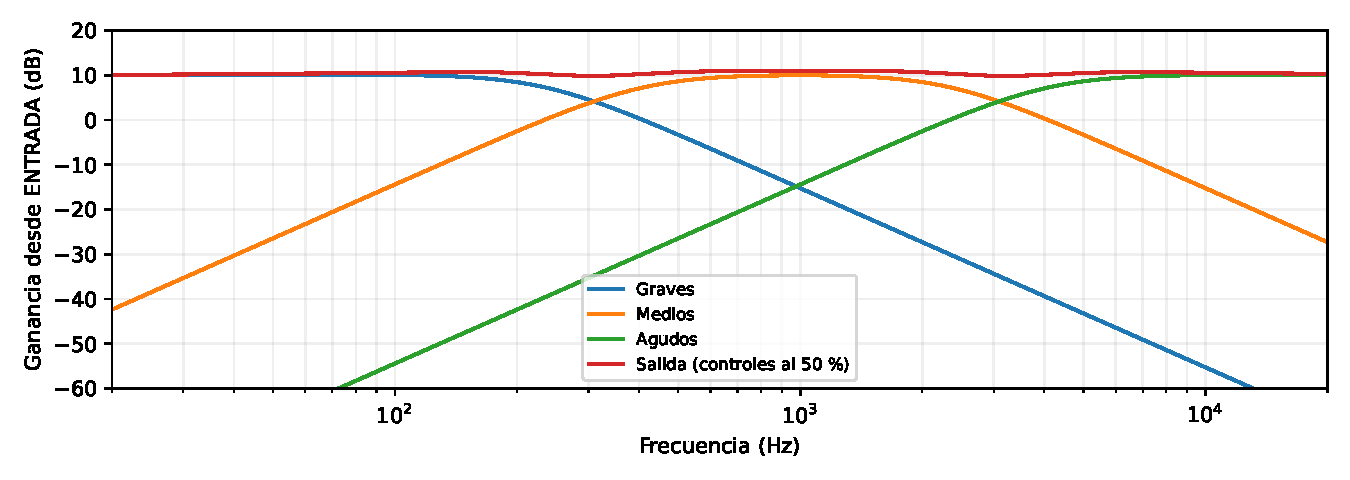
\includegraphics[width=\linewidth]{respuesta.pdf}
\siguientepagina
\section{10. Guion para presentar y registrar resultados}
\begin{enumerate}
\item \textbf{Mostrar la alimentación.} Medir +12 V y −12 V respecto a 0 V. Explicar que la señal alterna oscila alrededor de tierra.
\item \textbf{Mostrar la entrada y PRE.} A 1 kHz, comparar 100 mVpp con aproximadamente 320 mVpp. Explicar la ganancia no inversora.
\item \textbf{Mostrar las tres bandas.} Repetir 100 Hz, 1 kHz y 8 kHz. Identificar la salida dominante y guardar una captura de cada caso.
\item \textbf{Mostrar el control.} Mover CH4 a SALIDA. A 100 Hz, bajar RV1 y observar que cae la salida; repetir con RV2 a 1 kHz y RV3 a 8 kHz. Las otras ramas siguen contribuyendo, por lo que bajar una banda no obliga a obtener cero absoluto.
\item \textbf{Explicar la mezcla.} Mostrar MW y MI si hace falta: el inversor de medios cambia la polaridad. El sumador combina las tres señales con sus fases.
\item \textbf{Opcional: música.} Apagar o desconectar el generador; conectar una fuente de audio y un parlante activo. Empezar con volumen bajo y comprobar que EQ no presenta recorte.
\end{enumerate}

\begin{tabularx}{\linewidth}{lXXXX}\toprule Prueba & Entrada Vpp & Graves Vpp & Medios Vpp & Agudos Vpp\\\midrule
100 Hz & & & & \\[5mm]
1 kHz & & & & \\[5mm]
8 kHz & & & & \\[5mm]\bottomrule\end{tabularx}
Registrar también SALIDA con controles al 50 \% y con cada banda a mínimo/máximo. Conservar fotos del montaje y capturas con frecuencia, escala y Vpp visibles.

\section{Si algo no funciona}
\begin{itemize}
\item \textbf{Todas las salidas fallan:} revisar rieles, punto medio, pin 8/pin 4 y tramos interrumpidos de protoboard.
\item \textbf{Una salida queda cerca de un riel:} revisar realimentación al pin −, pinout y puentes temporales; probar otro TL072 ya verificado.
\item \textbf{Frecuencia incorrecta:} revisar códigos: 103 = 10 nF; 104 = 100 nF; 473 = 47 nF; 472 = 4,7 nF.
\item \textbf{Oscilación o señal gruesa:} acortar realimentaciones, acercar desacoples, separar entrada y salida; usar muelle de masa de sonda cuando sea posible.
\item \textbf{Recorte:} bajar la amplitud de entrada; no aumentar la fuente para corregir un error de cableado.
\end{itemize}
\section{Referencia y archivos}
Pinout y alimentación: \href{https://www.ti.com/lit/ds/symlink/tl072.pdf}{Texas Instruments, TL07xx, variante TL072CP clásica (no TL072H)}. Conexión serie de la fuente: consultar el manual UNI-T UDP3305S-E. El archivo \texttt{verificacion.cir} y las tablas CSV acompañan esta guía. La simulación comprueba la respuesta nominal de la red; el montaje físico todavía debe verificarse con las pruebas anteriores.
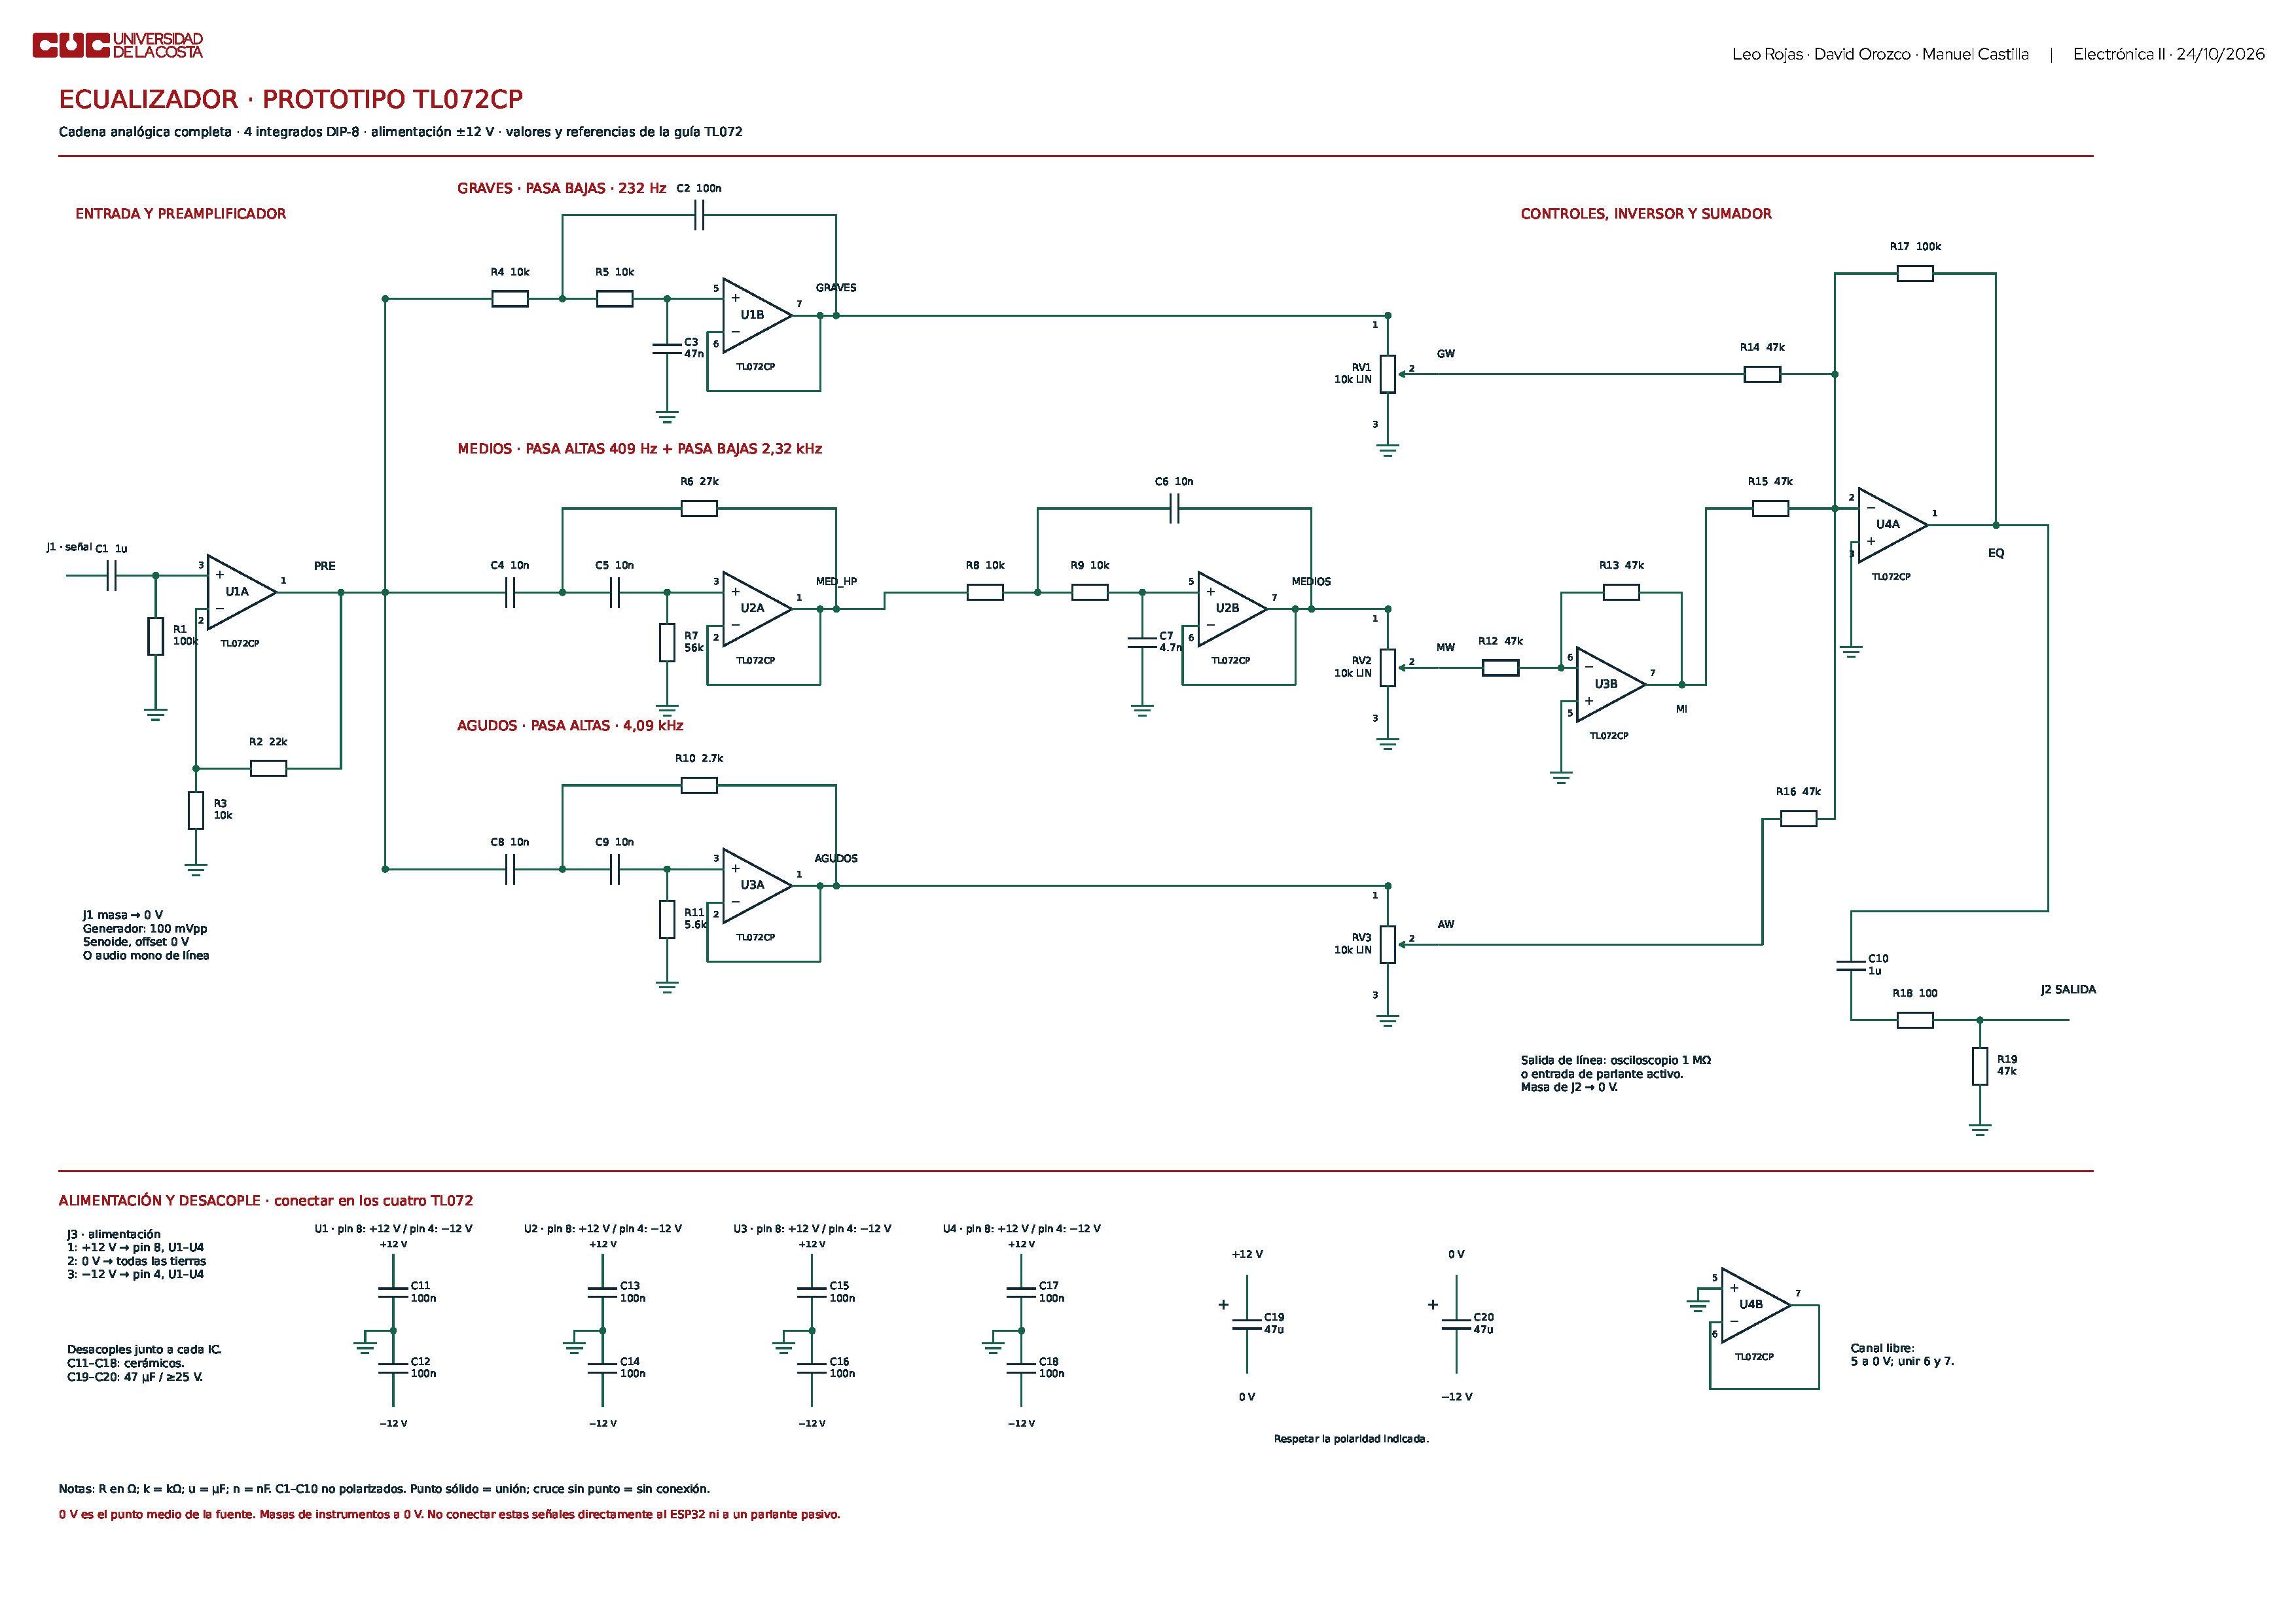
\includepdf[pages=-,fitpaper=true]{../prototipo-tl072/esquema-completo-TL072.pdf}
\end{document}
